\documentclass[11pt,a4paper]{jsarticle}
%

\usepackage{amsmath,amssymb}
\usepackage{bm}
\usepackage[dvipdfmx]{color}
\usepackage[dvipdfmx]{graphicx}
\usepackage{ascmac}
\usepackage{listings, jlisting}
\lstset{%
  basicstyle={\small},%
  identifierstyle={\small},%
  commentstyle={\small\itshape},%
  keywordstyle={\small\bfseries},%
  ndkeywordstyle={\small},%
  stringstyle={\small\ttfamily},
  frame={tb},
  breaklines=true,
  columns=[l]{fullflexible},%
  numbers=none,%
  xrightmargin=0zw,%
  xleftmargin=3zw,%
  numberstyle={\scriptsize},%
  stepnumber=1,
  numbersep=1zw,%
  lineskip=-0.5ex%
}


%
\setlength{\textwidth}{\fullwidth}
\setlength{\textheight}{40\baselineskip}
\addtolength{\textheight}{\topskip}
\setlength{\voffset}{-0.2in}
\setlength{\topmargin}{0pt}
\setlength{\headheight}{0pt}
\setlength{\headsep}{0pt}

%
\newcommand{\divergence}{\mathrm{div}\,}  %ダイバージェンス
\newcommand{\grad}{\mathrm{grad}\,}  %グラディエント
\newcommand{\rot}{\mathrm{rot}\,}  %ローテーション
%
\title{チャレンジサイト・メカニックカモノハシ2019\\マイクロマウスシミュレータの環境設定}
\author{ER17045 立道壱太郎}
\date{\today}
\begin{document}
\maketitle
%
%
\section{この資料について}
メカニックカモノハシではマイクロマウス大会に参加することでメンバーの技術向上を図ります。
開発時にはシミュレータを多用するので


\subsection{Ubuntu・ROSについて}
Ubuntu・ROSのを使うことで、より楽に開発できます。
\subsubsection{Ubuntuとは?}
UbuntuとはDebian系のLinux OSの一種で、開発者・研究者向けのOSです

Windowsでは無いので、ExcelやWordを始めとするWindowsのソフトを使用することは出来ません。
しかし、互換(パクリ)ソフトが用意されていたり、Linux版が存在したり、Windowsソフトが動く仕組み(Wine)
などがあるので特に困ることはありません。

また、Windowsのようにマウスで操作する事(GraphicalUserInterface)も可能ですが、キーボードで操作する事(CharacterUserInterface)も可能です。

以上の事から世界中で多くの開発者が利用しており、
わからないことがあっても、インターネットで検索すれば大体解決出来ます。


\subsubsection{ROSとは?}
ROSとはRobotOperationSystemの略です。「OS」と付いていますが、WindowsやUbuntuのようなものでは無く、
ロボットを開発するためのライブラリや開発環境の総称と思えば良いと思います。

ROSは世界中の開発者・研究者が利用しており、
ROSを使うことにより彼らが制作したプログラムを再利用することができます。
(再利用しやすい仕組みになっている)



\newpage
\subsection{WindowsとUbuntuのデュアルブート環境を構築する}
これからUbuntuをインストールしますが、Windowsが消えてしまうと困る(Windowsを使う授業が受けられない)ので、デュアルブート環境(1つのPCが2つのOSを持つこと)にしてWindowsとUbuntuそれぞれを利用できるようにします。

\subsection{データのバックアップ}
手順道理進めれば、データは消えませんが、万が一消えてしまった時のためにバックアップを取ります。
USBメモリを2つ用意してください。

1つめのUSBメモリには授業データや写真など、消えると困るデータを「全て」入れてください

2つめのUSBメモリはWindowsが消えて、かつ認証キーがわからない時用の回復メモリにしますが、今回はアドバイザ教授の長坂先生から認証キーを貰えるので、作る必要はありません。よって手順も書きません。

\subsection{Ubuntuのインストール}
「Windows Ubuntu デュアルブート」と調べればいくらでも出てきます。

\color{red}
しかし、注意点が3つあります。
\begin{itemize}
  \item インターネット接続状態で行う(有線接続が確実)
  \item Updateも一緒に行う。\\サードパーティ製のソフトウェアをインストールする。\\という旨の2つの選択肢にチェックを入れる。
  \begin{figure}[h]
    \begin{center}
      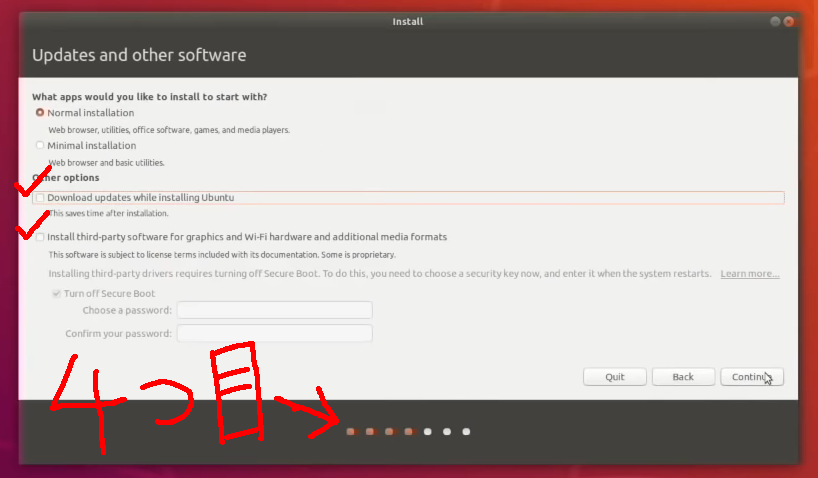
\includegraphics[width=128mm]{./install_caution.png}
    \end{center}
    \caption{}
    \label{graph3}
  \end{figure}
  \item 16.04LTSか18.04LTSをインストールする。
\end{itemize}



\color{black}

参考文献(このPDFの一番下)にいくつかURLを載せておきます。


%\lstinputlisting[caption=moving\_mouse.py,label=moveing_mouse,numbers=left]{./../script/chapters/1/moving_mouse.py}


\begin{thebibliography}{99}
\bibitem{install_ubuntu16} Windows10とUbuntu16.04のデュアルブート環境構築\\https://qiita.com/medalotte/items/4bb5cfa709e93d044f1c
\bibitem{install_ubuntu18} Windows10とUbuntu18.04をデュアルブートする.\\https://qiita.com/yo\_kanyukari/items/2a944a300db22482c696
\end{thebibliography}%
%
\end{document}
